%
% LulzBot Clonedel.tex
%
% History of LulzBot Printers
%
% Copyright (C) 2014, 2015 Aleph Objects, Inc.
%
% This document is licensed under the Creative Commons Attribution 4.0
% International Public License (CC BY-SA 4.0) by Aleph Objects, Inc.
%

\section{LulzBot Clonedel Molds}
The LulzBot Clonedel parts themselves were primarily poured from silicon molds.

\begin{figure}[h!]
\thisfloatpagestyle{empty}
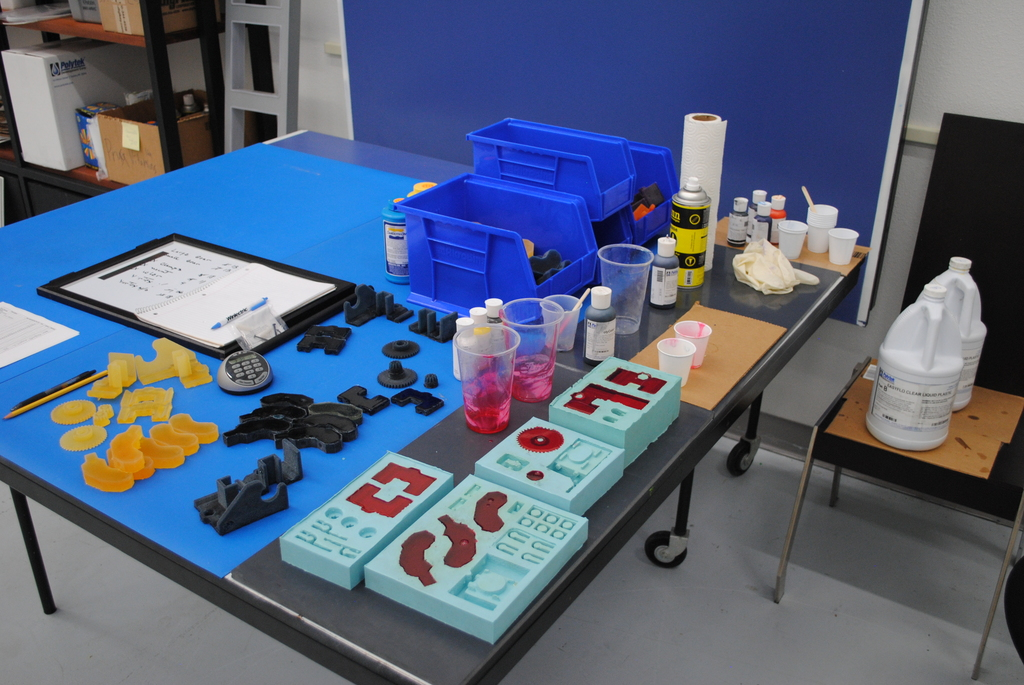
\includegraphics[keepaspectratio=true,height=0.40\textheight,width=1.00\textwidth,angle=0]{clonedel/table-layout.jpg}
 \caption{LulzBot Clonedel production ping pong table.}
 \label{fig:clonedel-table-layout}
\end{figure}

\begin{figure}[h!]
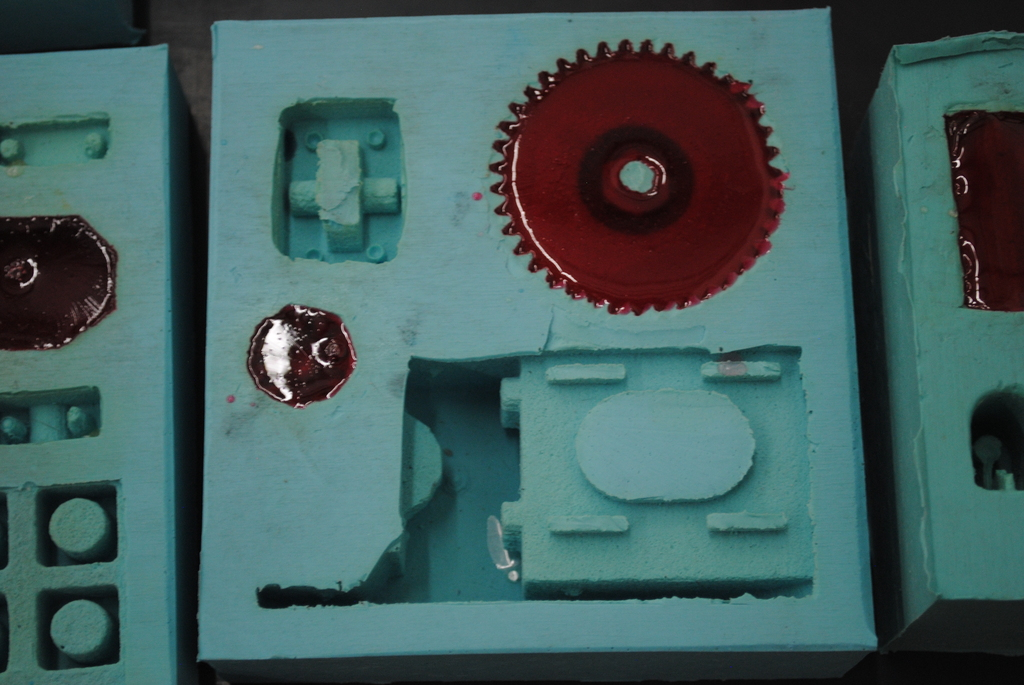
\includegraphics[keepaspectratio=true,height=0.40\textheight,width=1.00\textwidth,angle=0]{clonedel/gear-pour.jpg}
 \caption{LulzBot Clonedel gears in the silicon mold.}
 \label{fig:clonedel-gear-pour}
\end{figure}

\begin{figure}[h!]
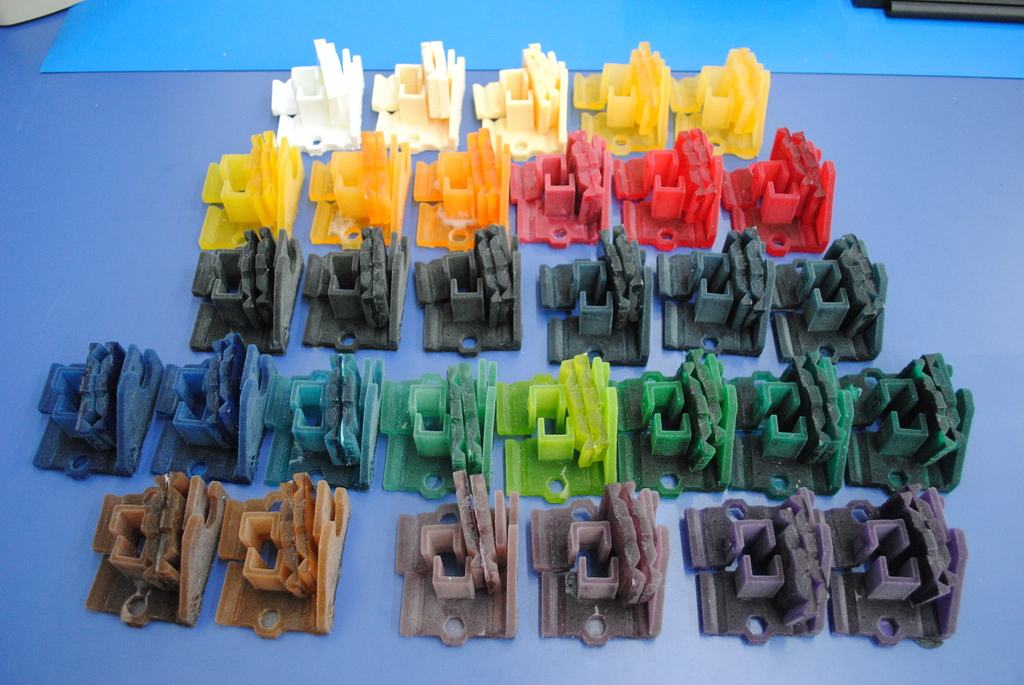
\includegraphics[keepaspectratio=true,height=0.40\textheight,width=1.00\textwidth,angle=0]{clonedel/clamps.jpg}
 \caption{LulzBot Clonedel molded parts.}
 \label{fig:clonedel-clamps}
\end{figure}

\begin{figure}[h!]
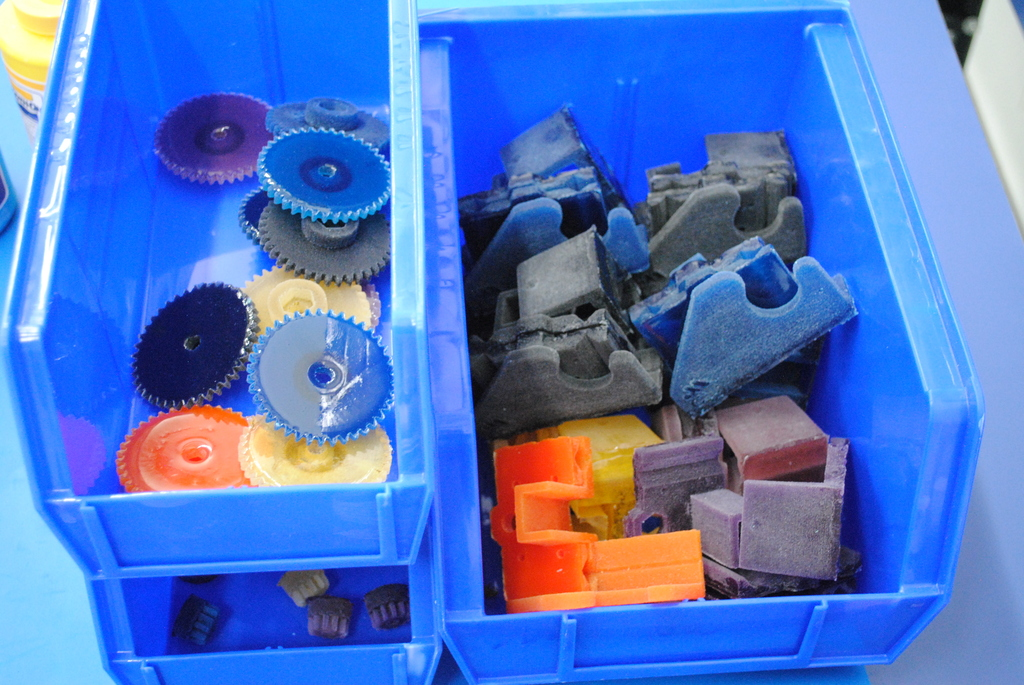
\includegraphics[keepaspectratio=true,height=0.40\textheight,width=1.00\textwidth,angle=0]{clonedel/gears-parts.jpg}
 \caption{LulzBot Clonedel molded gears.}
 \label{fig:clonedel-gears-parts}
\end{figure}

